\documentclass[11pt]{article}

\usepackage{amsmath}
\usepackage{amssymb}
\usepackage{array}
\usepackage{geometry}
\usepackage{enumitem}
\usepackage{float}
\usepackage{cancel}
\usepackage{graphicx}
\usepackage[labelformat=empty]{caption}

\geometry{
	a4paper,
 	left=20mm,
 	top=20mm,
}

\setlength{\parindent}{0pt}

\begin{document}

\section{Mengen}

\begin{description}[labelindent=16pt,style=multiline,leftmargin=6cm, noitemsep]
	\item[Obere/Untere Schranke:] $\exists b \in \mathbb{R}\ \forall a\in A:\ a \leq b$, $\exists c \in \mathbb{R}\ \forall a\in A:\ a \geq c$
	\item[Supremum:] kleinste obere Schranke $\sup A$
	\item[Infimum:] gr{\"o}sste untere Schranke $\inf A$
	\item[Maximum/Minimum:] $\sup A \in A$, $\inf A \in A$
\end{description}

\section{Komplexe Zahlen}

\subsection{Polarform}

\begin{minipage}[c]{0.5\textwidth}
\centering
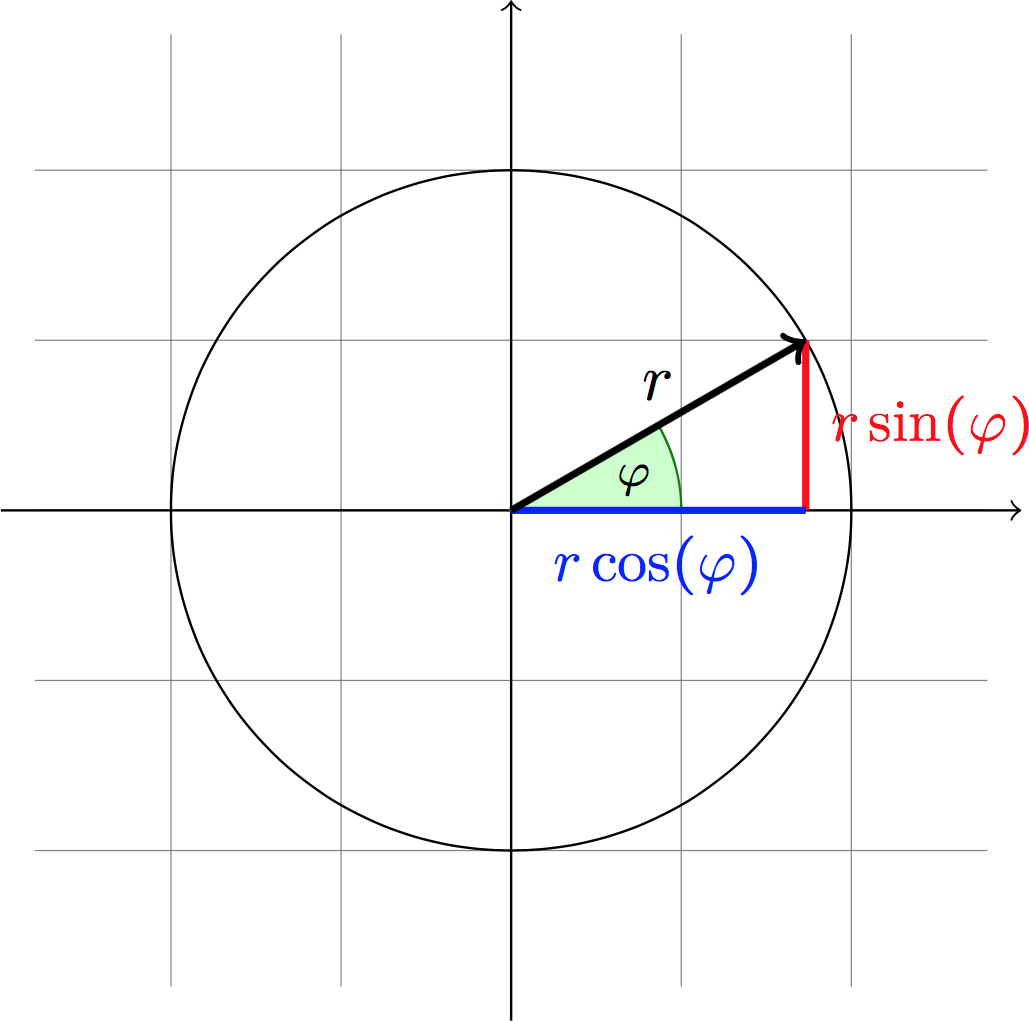
\includegraphics[width=\linewidth,keepaspectratio=true]{images/polarform}
\end{minipage}
%
\begin{minipage}[c]{0.5\textwidth}
\begin{equation*}
\begin{split}
	z & = x + iy = r(\cos(\varphi) + i\sin(\varphi)) = re^{i\varphi} \\
	r & = |z| = \sqrt{x^2 + y^2} \\
	\varphi & = \arctan(\frac{y}{x}) =  \\
	x & = r\cos(\varphi) \\
	y & = r\sin(\varphi) \\
	zw & = (re^{i\varphi})\cdot(se^{i\psi}) = rse^{i(\varphi + \psi)} \\
	\sqrt[q]{z} & = \sqrt[q]{s}e^{i\phi}\text{, wobei }\phi = \frac{\varphi}{q} \mod \frac{2\pi}{q} \\
	e^{i(\frac{\pi}{2} + 2\pi k)} & = i,\ e^{i\pi} = 1, \ e^{-i\pi} = -1
\end{split}
\end{equation*}
\end{minipage}

\subsection{Identit{\"a}ten}

\begin{equation*}
\begin{split}
	\overline{z} & = x - iy\\
	z^{-1} & = \frac{\overline{z}}{|z|^2} \\
	(a,b) \cdot (c, d) & = (ac-bd, ad+bc) \\
	i & = \sqrt{-1}\\
	i^2 & = -1 \\
	|z|^2 & = z\overline{z} \\
	|zw|^2 & = (zw) \cdot \overline{(zw)} = |z|^2|w|^2
\end{split}
\end{equation*}

\section{Trigonometrie}

\begin{equation*}
\begin{split}
	\sin(0) = 0,\ \sin(\frac{\pi}{4}) = \frac{\sqrt{2}}{2},\ \sin(\frac{\pi}{2}) & = 1,\ \sin(\pi) = 0,\ \sin(\frac{3\pi}{4}) = \frac{\sqrt{2}}{2}\\
	\cos(0) = 1,\ \cos(\frac{\pi}{4}) = \frac{\sqrt{2}}{2},\ \cos(\frac{\pi}{2}) & = 0,\ \cos(\pi) = -1,\ \cos(\frac{3\pi}{4}) = -\frac{\sqrt{2}}{2}\\
\end{split}
\end{equation*}

\begin{equation*}
\begin{split}
	\tan(x) & = \frac{\sin(x)}{\cos(x)} \\
	\sin(2x) & = 2\sin(x)\cos(x) \\
	\sin(\alpha + \beta) & = \sin(\alpha)\cos(\beta) + \cos(\alpha)\sin(\beta) \\
	\cos(\alpha + \beta) & = \cos(\alpha)\cos(\beta) + \sin(\alpha)\sin(\beta) \\
	\cos^2(x) & = \frac{1 + \cos(2x)}{2} \\
	\sin^2(x) + \cos^2(x) & = 1
\end{split}
\end{equation*}

\section{Grenzwert}

\subsection{Dominanz}

\begin{equation*}
\begin{split}
	\text{F{\"u}r}\ x \to +\infty:\quad & ... < \log(\log(x)) < \log(x) < x^\alpha < \alpha^x < x! < x^x \\
	\text{F{\"u}r}\ x \to 0:\quad & ... < \log(\log(x)) < \log(x) < (\frac{1}{x})^\alpha \\
\end{split}
\end{equation*}

\subsection{Tipps}

\begin{equation*}
\begin{split}
	\lim_{x \to a} \frac{\sin \odot}{\odot} & = 1\ \text{mit}\ \odot \xrightarrow{\: x \to a \: } 0 \\ 
	\lim_{x \to a} (1 + \frac{1}{\odot})^\odot & = e\ \text{mit}\ \odot \xrightarrow{\: x \to a \: } \infty \\ 
	\lim_{x \to a} (1 + \odot)^\frac{1}{\odot} & = e\ \text{mit}\ \odot \xrightarrow{\: x \to a \: } 0 \\ 
\end{split}
\end{equation*}

\subsection{Wurzeltrick}

\begin{equation*}
	\lim_{x\to\infty} \sqrt{\alpha}+\beta = \lim_{x\to\infty}(\sqrt{\alpha}+\beta)\frac{\sqrt{\alpha}-\beta}{\sqrt{\alpha}-\beta}
\end{equation*}

\subsection{$e^{\log(x)}$-Trick}

\subsubsection*{Anforderung}

Term der Form $f(x)^{g(x)}$ mit Grenzwert "$0^0$", "$\infty^0$" oder "$1^\infty$" f{\"u}r $x \to 0$

\subsubsection*{Vorgehen}

\begin{equation*}
	\lim_{x\to a}f(x)^{g(x)} = \lim_{x\to a}e^{g(x) \cdot \log(f(x))}
\end{equation*}

\subsection{Satz von Bernoulli-de l'H{\^o}pital}

\subsubsection*{Anforderung}

Term der Form $\frac{f(x)}{g(x)}$ mit Grenzwert entweder "$\frac{0}{0}$" oder "$\frac{\infty}{\infty}$" mit $g'(x) \neq 0$. \\
Falls die Grenzwerte $0 \neq \infty$ verschieden sind, kann man umformen: $\frac{f(x)}{\frac{1}{g(x)}}$.

\subsubsection*{Vorgehen}

\begin{equation*}
	\lim_{x\to a}\frac{f(x)}{g(x)} = \lim_{x\to a}\frac{f'(x)}{g(x)}
\end{equation*}

\section{Folgen und Reihen}

\section{Differenzialrechnung}

Eine stetige Funktion ist differenzierbar, falls der Grenzwert $f'(x_0)$ existiert:

\begin{equation*}
	f'(x_0) := \lim_{x\to x_0}\frac{f(x) - f(x_0)}{x-x_0}
\end{equation*}

\subsection{Umkehrsatz}

\begin{equation*}
	(f^{-1})'(y) = \frac{1}{f'(x)}
\end{equation*}

\subsection{Mittelwertsatz}

\begin{equation*}
	f'(c) = \frac{f(b) - f(a)}{b - a}
\end{equation*}

\subsection{Taylorpolynom}

Das Taylorpolynom $m$-ter Ordnung von $f(x)$ an der Stelle $x=a$
\begin{equation*}
	P^a_m(x) := f(a) + f'(a)(x-a) + \frac{1}{2}f''(a)(x-a)^2 + ... + \frac{1}{m!} f^{(m)}(a)(x-a)^m
\end{equation*}

mit dem Fehlerterm $R^a_m(x)$, wobei $\xi$ zwischen $a$ und $b$ liegt:
\begin{equation*}
	R^a_m(x) = \frac{f^{(m+1)}(\xi)}{(m+1)!}(x+a)^{m+1},\ \text{wobei}\ f(x) = P^a_m(x) + R^a_m(x)
\end{equation*}

\section{Integration}

\subsection{Elementare Integrale}

\begin{table}[H]
\centering
\begin{tabular}{|l|l|}
\hline
$f(x)$ & $F(x)$ \\ \hline
$x^\alpha$ & $\frac{x^{\alpha+1}}{\alpha+1} + C$ \\ \hline
$\frac{1}{x}$ & $\log (x) + C$ \\ \hline
$\frac{1}{x^2}$ & $\frac{1}{x} + C$ \\ \hline
$\sin(x)$ & $-\cos(x) + C$ \\ \hline
$\cos(x)$ & $\sin(x) + C$ \\ \hline
\end{tabular}
\end{table}

\subsection{Regeln}

\begin{equation*}
\begin{split}
	\textbf{Direkter Integral}\quad & \int f(g(x))g'(x)\ dx = F(g(x)) \\
	\textbf{Partielle Integration}\quad & \int f' \cdot g\ dx = f \cdot g - \int f \cdot g'\ dx \\
	\textbf{mit Polynomen}\quad & \int\frac{p(x)}{q(x)}\ dx \Rightarrow\ \text{Partialbruchzerlegung} \\
	\textbf{Substitution}\quad & \int_a^b f(\varphi(t))\varphi'(t)\ dt = \int_{\varphi(a)}^{\varphi(b)} f(x)\ dx\ \text{mit}\ x = \varphi(t)
\end{split}
\end{equation*}

\subsection{Tipps}

\begin{equation*}
\begin{split}
	\int\tan x\ dx & = \int\frac{\sin x}{\cos x}\ dx = -\log|\cos(x)| \\
	\int \frac{1}{x - \alpha} & = \log(x-\alpha) \\
\end{split}
\end{equation*}

\section{Differentialgleichungen}

\subsection{Grundbegriffe}

\begin{description}[labelindent=16pt,style=multiline,leftmargin=3.5cm, noitemsep]
	\item[Ordnung:] h{\"o}chste vorkommende Ableitung
	\item[linear:] alle $y$-abh{\"a}ngigen Terme kommen linear vor (keine Terme wie zum Beispiel $y^2$, $(y'')^3$, $\sin(y)$, $e^{y'}$)
	\item[homogen:] Gleichung ohne St{\"o}rfunktionen
	\item[St{\"o}rfunktion:] Term, der rein von der Funktionsvariablen $x$ abh{\"a}ngt
\end{description}

\subsection{Methoden}

\begin{table}[H]
\centering
\begin{tabular}{|p{5cm}|p{6cm}|p{3cm}|}
\hline
                                  	& \textbf{Problem} 							& \textbf{Anforderungen} 			\\ \hline
\textbf{Trennung der Variablen}   	& $y' = \frac{dy}{dx} = h(x) \cdot g(y)$ 	& 1. Ordnung			            \\ \hline
\textbf{Variation der Konstanten}	& $y' = \frac{dy}{dx} = h(x)y + b(x)$	 	& 1. Ordnung \filbreak inhomogen	\\ \hline
\textbf{Euler-Ansatz}				& $a_{n}y^{(n)} + a_{n-1}y^{(n-1)} + ... + a_{0}y = 0$	 	& n. Ordnung \filbreak linear \filbreak homogen	\\ \hline
\textbf{Direkter Ansatz}				& $a_{n}y^{(n)} + a_{n-1}y^{(n-1)} + ... + a_{0}y = b(x)$	& n. Ordnung \filbreak linear \filbreak inhomogen	\\ \hline

%\textbf{Substitution}				& $y' = h(\frac{y}{x})$ \filbreak $y' = h(ax + by + c)$ \filbreak $y' = h(\frac{ax + by + c}{dx + ey + f})$ \filbreak $y' = \frac{y}{x}h(xy)$ 																		& nicht direkt separierbar			\\ \hline
\end{tabular}
\end{table}

\subsubsection{Trennung der Variable}

\begin{equation*}
\begin{split}
	& y' + x \tan y = 0,\ y(0) = \frac{\pi}{2} \\
	\text{umformen}\quad & \frac{dy}{dx} = -x \tan y \\
	\textbf{konstante L{\"o}sungen}\quad & y(x) \equiv 0\ \text{erf{\"u}llt jedoch $y(0) \equiv \frac{\pi}{2}$ nicht} \\
	\text{Trennung}\quad & \frac{dy}{\tan y} = -x dx \\
	\text{integrieren}\quad & \int\frac{\cos y}{\sin y}dy = - \int xdx \Rightarrow \log|\sin y| = -\frac{x^2}{2} + C \\
	& \Rightarrow |\sin y| = e^Ce^{\frac{-x^2}{2}} \Rightarrow \sin y = \pm e^Ce^{\frac{-x^2}{2}} = Ce^{\frac{-x^2}{2}} \\
	\text{Anfangsbedingung gebrauchen}\quad & \sin(y(0)) = \sin (\frac{\pi}{2}) = 1 \Rightarrow C = 1 \\
	\textbf{L{\"o}sung}\quad & y(x) = \arcsin (e^{\frac{-x^2}{2}})
\end{split}
\end{equation*}

\subsubsection{Variation der Konstanten}

\begin{equation*}
	\textbf{Grundsatz:}\quad y(x) = y_\text{homo}(x) + y_p(x)
\end{equation*}

\begin{equation*}
\begin{split}
	& y' - y = 1,\ y(0) = 0 \\
	\text{homogener Ansatz}\quad & y' = y \\
	\textbf{konstante L{\"o}sungen}\quad & y(x) \equiv 0 \\
	\text{Trennung}\quad & \frac{dy}{y} = dx \Rightarrow \int\frac{dy}{y} = \int dx \Rightarrow \log|y| = x \\
	\textbf{homogene L{\"o}sung}\quad & y_\text{homo}(x) = Ae^x,\ A = e^C \in \mathbb{R} \\
	\text{partikul{\"a}rer Ansatz}\quad & y_p(x) = A(x)e^x \\
	\text{einsetzen}\quad & A'e^x + Ae^x - Ae^x = 1 \Rightarrow A' = e^{-x} \Rightarrow A(x) = \int e^{-x}\ dx = -e^{-x} \\
	\textbf{partikul{\"a}re L{\"o}sung}\quad & y_p(x) = -1 \\
	\textbf{L{\"o}sung}\quad & y(x) = Ae^x - 1\ \text{mit Anfangsbedingung}\ A = 1 \\
	& \Rightarrow y(x) = e^x - 1
\end{split}
\end{equation*}

%\subsubsection{Substitution}
%
%\begin{equation*}
%\begin{split}
%	& y' = h(\frac{y}{x})\ \text{ersetzt durch}\ z(x) = \frac{y(x)}{x} \Leftrightarrow y(x) = xz(x) \\
%	& \Rightarrow	y' = z + xz'
%\end{split}
%\end{equation*}

\subsubsection{Euler-Ansatz}

\begin{equation*}
\begin{split}
	& y'' - 2y' - 8y = 0,\ y(1) = 1, y'(1) = 0 \\
	\text{Euler-Ansatz}\quad & y(x) = e^{\lambda x} \\
	\text{einsetzen}\quad & \lambda^2 e^{\lambda x} - 2\lambda e^{\lambda x} - 8e^{\lambda x} = 0 \\
	\textbf{charakt. Polynom}\quad & \lambda^2 - 2\lambda - 8 = (\lambda - 4)(\lambda + 2) = 0 \\
	\text{Nullstellen}\quad & 4, -2 \\
	\textbf{allgemeine L{\"o}sung}\quad & y(x) = Ae^{4x} + Be^{-2x} \\
	\text{Anfangsbedingung gebrauchen}\quad & y(1) = Ae^4 + Be^{-2} = 1,\ y'(1) = 4Ae^4 - 2Be^{-2} = 0 \\
											& \Rightarrow A = \frac{1}{3}e^{-4}, B = \frac{2}{3}e^2 \\
	\textbf{L{\"o}sung}\quad & y(x) = \frac{1}{3}e^{4x-4} + \frac{2}{3}e^{2-2x}
\end{split}
\end{equation*}

\emph{Bemerkung:} Zu einer $m$-fachen Nullstelle $\lambda$ geh{\"o}ren die $m$ linear unabh{\"a}ngigen L{\"o}sungen $e^{\lambda x}$, $x\cdot e^{\lambda x}$, ... , $x^{m-1}\cdot e^{\lambda x}$. Zur $m$-fachen Nullstelle $\lambda = 0$ geh{\"o}ren die L{\"o}sungen $1$, $x$, ... , $x^{m-1}$.

\subsubsection{Direkter Ansatz}

\begin{equation*}
	\textbf{Grundsatz:}\quad y(x) = y_\text{homo}(x) + y_p(x)
\end{equation*}

\begin{table}[H]
\centering
\begin{tabular}{|l|l|l|}
\hline
\textbf{Inhomogener Term $b(x)$} & \textbf{Ansatz f{\"u}r $y_p(x)$}	& \textbf{zu bestimmen}		\\ \hline
Polynom				& $Ax^2 + Bx + C$			& $A$, $B$, $C$		\\ \hline
$c e^{k x}$ & $Ae^{kx}$					& $A$				\\ \hline
$c\sin(kx)$ oder $c\cos(kx)$ & $A\sin(kx) + B\cos(kx)$ & $A$, $B$ \\ \hline

\end{tabular}
\end{table}

\begin{equation*}
\begin{split}
	& y'' - y' + \frac{1}{4}y = \cos(x) \\
	\text{homogener}\quad & y'' + y' + \frac{1}{4}y = 0 \\
	\text{Euler-Ansatz anwenden}\quad & \lambda^2 + \lambda + \frac{1}{4} = (\lambda + \frac{1}{2})^2 = 0 \\
	\textbf{homogene L{\"o}sung}\quad &\Rightarrow y_\text{homo}(x) = Ae^{-\frac{x}{2}} + Bx \cdot e^{-\frac{x}{2}} \\
	\text{Ansatz w{\"a}hlen}\quad & y_p(x) = a\cos(x) + b\sin(x) \\
							  & \Rightarrow y_p'(x) = -a\sin(x) + b\cos(x),\  y_p''(x) = -a\cos(x) -b \sin(x) \\
	\text{Einsetzen}\quad & (-a + b + \frac{a}{4})\cos(x) + (-b -a + \frac{1}{4}b)\sin(x) = \cos(x) \\
	\text{Koeffizientenvergleich}\quad & -\frac{3}{4}a + b = 1,\ -a-\frac{3}{4}b = 0 \\
	\textbf{partikul{\"a}re L{\"o}sung}\quad & y_p(x) = -\frac{12}{25}\cos(x) + \frac{16}{25}\sin(x) \\
	\textbf{L{\"o}sung}\quad & y(x) = Ae^{-\frac{x}{2}} + Bx \cdot e^{-\frac{x}{2}} -\frac{12}{25}\cos(x) + \frac{16}{25}\sin(x)
\end{split}
\end{equation*}

\section{Wegintegral}

\subsection{Standard Methode}

\begin{equation*}
	\textbf{Grundsatz:}\quad \int_\gamma \vec{v}\cdot d\vec{s} := \int_a^b \vec{v}(\vec{\gamma}(t)) \cdot \dot\vec{\gamma}(t)\ dt
\end{equation*}

\begin{equation*}
\begin{split}
	& \vec{v} = \binom{y}{0},\ \gamma:[0, 2\pi] \mapsto \mathbb{R}^2,\ t \mapsto \binom{t -\sin(t)}{1-\cos(t)} \\
	\text{parametrisieren}\quad & \text{hier bereits gegeben} \\
	\text{$\gamma$ ableiten}\quad & \dot\gamma = \binom{1-\cos(t)}{\sin(t))} \\
	\text{in Formel einsetzen}\quad & \int_\gamma \vec{v} \cdot d\vec{s} = \int_0^{2\pi} \binom{1-\cos(t)}{0}\cdot\binom{1-\cos(t)}{\sin(t)}\ dt \\
	&= \int_0^{2\pi} (1-\cos(t))^2\ dt = \int_0^{2\pi} (1-2\cos(t)+\cos^2(t))\ dt \\
	\textbf{L{\"o}sung}\quad & 2\pi - 0 + \pi = 3\pi
\end{split}
\end{equation*}

\subsection{In Potenzialfeldern}

\paragraph{Anforderung:} Das Vektorfeld $\vec{v}$ ist \textbf{konservativ}. Es existiert ein Potenzial.

\begin{equation*}
	\textbf{Grundsatz:}\quad\int_\gamma \vec{v} \cdot d\vec{s} = \Phi(\text{Ende}) - \Phi(\text{Anfang})
\end{equation*}

\begin{equation*}
\begin{split}
	& \vec{v} = \binom{e^{xy}(1 + xy)}{e^{xy}x^2},\ \text{Kreisbogen von } (1,0)\ \text{nach}\ (-1,0) \\
	\text{gleichsetzen:}\quad & \vec{v} = \binom{e^{xy}(1 + xy)}{e^{xy}x^2} \overset{!}{=} \binom{\frac{\partial\Phi}{\partial x}}{\frac{\partial\Phi}{\partial y}} = \nabla\Phi \\
	& \frac{\partial\Phi}{\partial y} = e^{xy}x^2 \Rightarrow \Phi = \int e^{xy}x^2\ dy = xe^{xy} + C(x) \\
	\text{ableiten:}\quad & \frac{\partial\Phi}{\partial x} = e^{xy} + xye^{xy} + C' \overset{!}{=} e^{xy} + xye^{xy} \\
	& \Rightarrow C' = 0 \Rightarrow C = \text{const.} \\
	\textbf{Potenzial:}\quad & \Phi = xe^{xy} + \text{const.} \\
	\textbf{L{\"o}sung:}\quad & \int_\gamma \vec{v} \cdot d\vec{s} = \Phi(-1,0) - \Phi(1,0) = -1 + C -1 - C = 2
\end{split}
\end{equation*}

\subsection{Satz von Green}

\paragraph{Anforderung:} Der Rand muss im positiven mathematischen Sinn umlaufen werden (d.h. im Gegenuhrzeigersinn)

\begin{equation*}
	\textbf{Grundsatz:}\quad\int_{\gamma = \partial C} \vec{v} \cdot d\vec{s} = \int_C (\frac{\partial v_2}{\partial x}-\frac{\partial v_1}{\partial y})\ dxdy
\end{equation*}

\begin{equation*}
\begin{split}
	& \vec{v} = \binom{x+y}{y},\ \text{Kreisbogen mit Radius $1$ um $(0,0)$} \\
	\text{Rotation berechnen:}\quad & rot(\vec{v}) = \frac{\partial v_2}{\partial x}-\frac{\partial v_1}{\partial y} = 0 -1 = -1 \\
	\text{Normalbereich:}\quad & E = \{(x,y) \in \mathbb{R}^2 | x^2 + y^2 \leq 1 \} \\
	\text{in Formel einsetzen:}\quad & \int_\gamma \vec{v} \cdot d\vec{s} = \int_E -1\ dxdy = -\mu(E) = -\pi
\end{split}
\end{equation*}

\section{Fl{\"a}chenintegral}

\subsection{Normalbereich}

\begin{equation*}
\begin{split}
	\textbf{Grundsatz:}\quad & \Omega = \{(x,y) \in \mathbb{R}^2| a \leq x \leq b, f(x) \leq y \leq g(x)\} \\
	& \int_\Omega F\ d\mu = \int_a^b dx \int_{f(x)}^{g(x)} dy\ F(x,y)
\end{split}
\end{equation*}

\begin{equation*}
\begin{split}
	& \int_\Omega xy\ d\mu,\ \Omega = \{(x,y) \in \mathbb{R}^2| y \geq x^2, x \geq y^2 \} \\
	\text{als Normalbereich schreiben:}\quad & \Omega = \{(x,y) \in \mathbb{R}^2| 0 \leq x \leq 1, x^2 \leq y \leq \sqrt{x}\} \\
	\text{in Formel einsetzen:}\quad & \int_\Omega xy\ d\mu = \int_0^1 dx\int_{x^2}^{\sqrt{x}} dyxy = \int_0^1 dx\ x \Big[\frac{y^2}{2}\Big]_{x^2}^{\sqrt{x}} \\
	& = \int_0^1 \Big(\frac{x^2}{2}-\frac{x^5}{2}\Big)dx = \frac{1}{12} \\
\end{split}
\end{equation*}

\subsection{Satz von Green}

\begin{equation*}
	\textbf{Grundsatz:}\quad \mu(C) = \int_{\gamma = \partial C} \vec{v} \cdot d\vec{s}\text{, falls}\ rot(\vec{v}) = 1
\end{equation*}

\begin{equation*}
\begin{split}
	& \text{Fl{\"a}cheninhalt der Ellipse $E$, berandet durch} x = a\cos(\theta),\ y = b\sin(\theta) \\
	\text{Rand parametrisieren:}\quad & \gamma: [0, 2\pi] \mapsto \mathbb{R}^2,\ \theta \mapsto \binom{a\cos(\theta)}{b\sin(\theta)} \\
	\text{Vektorfeld ausw{\"a}hlen:}\quad & \vec{v}_1 = \binom{0}{x}\ \text{oder}\ \vec{v}_2 = \binom{-y}{0} \\
	\textbf{Wegintegral ausrechnen}\quad & \mu(E) = \pi ab
\end{split}
\end{equation*}

\section{Kurvendiskussion}

\subsection{Extrema/Minima}

\paragraph{Kritischer Punkt:} $p_0 \in \Omega$ f{\"u}r welchen $df(p_0)$ nicht den maximalen Rang besitzt, also falls $Rang(df(p_0)) < \min{n, m}$.

\end{document}
